%!TEX TS-program = xelatex
%!TEX encoding = UTF-8 Unicode

\documentclass[12pt]{extarticle}
% extarticle is like article but can handle 8pt, 9pt, 10pt, 11pt, 12pt, 14pt, 17pt, and 20pt text

\def \ititle {Origins of Mind}
 
\def \isubtitle {Lecture 08}
 
\def \iauthor {Stephen A. Butterfill}
\def \iemail{s.butterfill@warwick.ac.uk}
\date{}

%for strikethrough
\usepackage[normalem]{ulem}

\input{$HOME/Documents/submissions/preamble_steve_handout}

%logic symbol \leftmodels
\usepackage{MnSymbol}

%\bibpunct{}{}{,}{s}{}{,}  %use superscript TICS style bib
%remove hanging indent for TICS style bib
%TODO doesnt work
\setlength{\bibhang}{0em}
%\setlength{\bibsep}{0.5em}


%itemize bullet should be dash
\renewcommand{\labelitemi}{$-$}

\begin{document}

\raggedcolumns

\begin{multicols*}{3}

\setlength\footnotesep{1em}


\bibliographystyle{newapa} %apalike

%\maketitle
%\tableofcontents




%--------------- 
%--- start paste

\def \ititle {Logic I}
 
\def \isubtitle {Fast Lecture 04}
 
\begin{center}
 
{\Large
 
\textbf{\ititle}: \isubtitle
 
}
 
 
 
\iemail %
 
\end{center}
 
Readings refer to sections of the course textbook, \emph{Language, Proof and Logic}.
 
 
 
\section{Everything Is Broken}
 
\emph{Reading:} §9.1, §9.2
 
Everything is broken: ∀x Broken(x)
 
Something is broken: ∃x Broken(x)
 
 
 
\section{∃Elim}
 
\emph{Reading:} §12.2, §13.2
 
\begin{center}
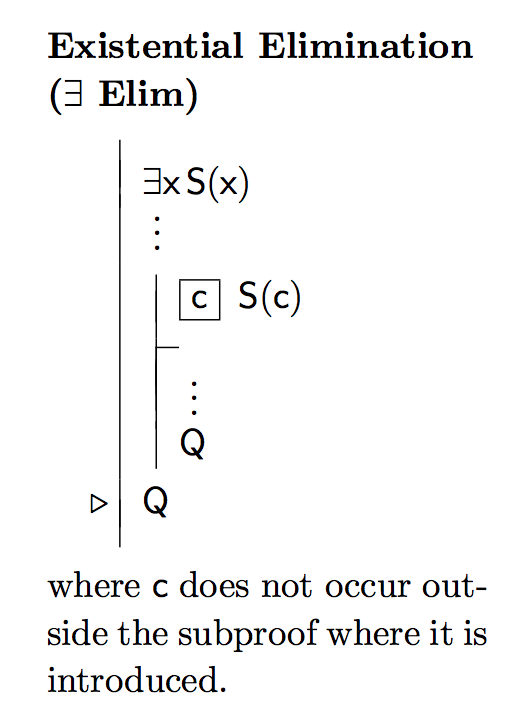
\includegraphics[scale=0.3]{img/rule_existential_elim.png}
\end{center}
\begin{center}
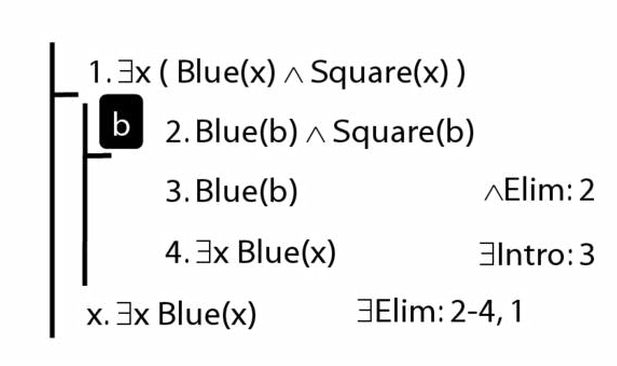
\includegraphics[scale=0.3]{img/proof_existential_elim.png}
\end{center}
\begin{minipage}{\columnwidth}
 
Note this restriction on the use of ∃Elim:
 
\begin{center}
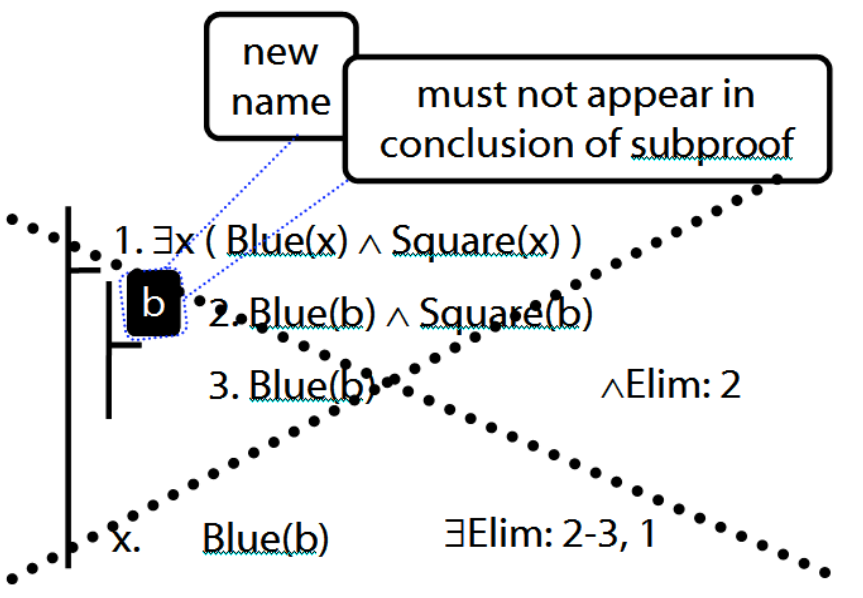
\includegraphics[scale=0.3]{img/proof_existential_elim_incorrect.png}
\end{center}
\end{minipage}
 
 
 
\section{All Squares Are Blue (Fast Version)}
 
\emph{Reading:} §9.2, §9.3, §9.5
 
\begin{minipage}{\columnwidth}
 
\emph{∃ and ∧ work together}
 
Some square is blue:
 
∃x ( Square(x) ∧ Blue(x) )
 
Some of my things are broken:
 
∃x ( Belongs(a,x) ∧ Broken(x) )
 
\end{minipage}
 
\begin{minipage}{\columnwidth}
 
\emph{∀ and → work together}
 
All squares are blue:
 
∀x ( Square(x) → Blue(x) )
 
All my things are broken:
 
∀x ( Belongs(a,x) → Broken(x) )
 
\end{minipage}
 
 
 
\section{What does ∀ mean?}
 
\emph{Reading:} §9.4
 
We give the meaning of ∀ by specifying what it takes for a sentence containing ∀ to be true:
 
\begin{enumerate}
 
\item Give every object a name.
 
\item For each name in turn, create a new sentence like this: delete the quantifier and replace all instances of the variable it binds with that name.
 
\item If ALL of the new sentences are true, so is the original sentence.
 
\end{enumerate}
 
 
\begin{minipage}{\columnwidth}

\section{∀Intro}
 
\emph{Reading:} §12.1, §12.3, §13.1
 
\begin{center}
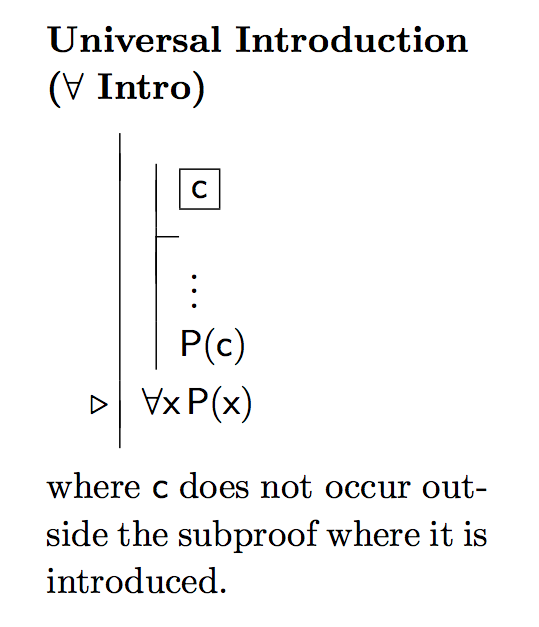
\includegraphics[scale=0.3]{img/rule_universal_intro.png}
\end{center}
\begin{center}
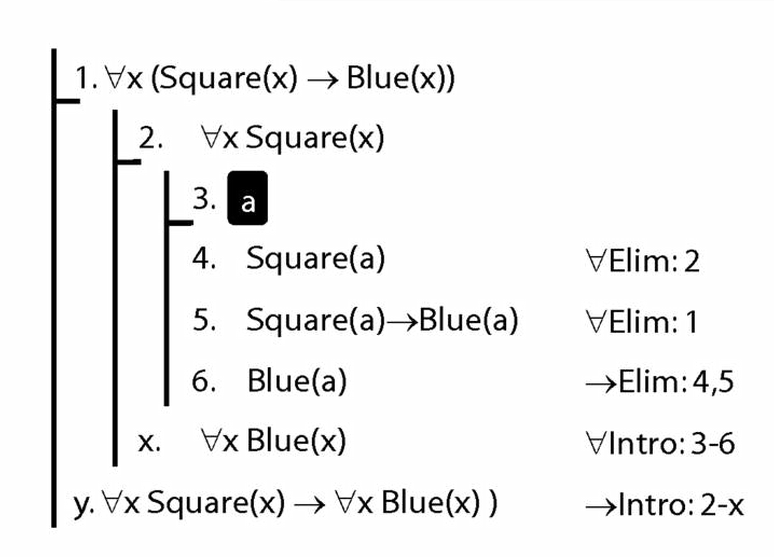
\includegraphics[scale=0.3]{img/proof_universal_intro.png}
\end{center}
\end{minipage}


\begin{minipage}{\columnwidth}
 
Why is this proof incorrect?
 
\begin{center}
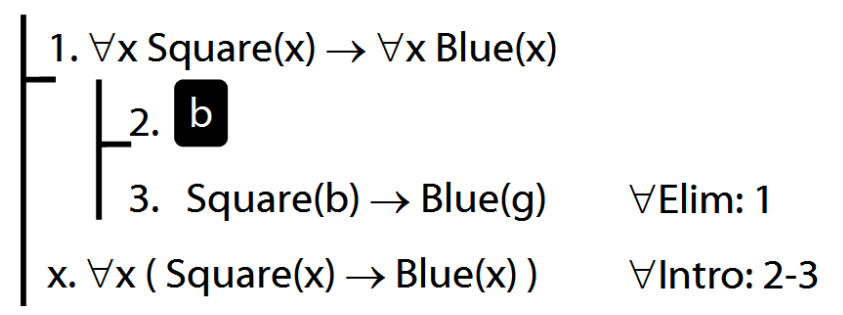
\includegraphics[scale=0.3]{img/proof_universal_intro_incorrect.png}
\end{center}
\end{minipage}
 
 
 
\section{Summary of Quantifier Rules}
 
\emph{Reading:} §13.1, §13.2
 
\begin{center}
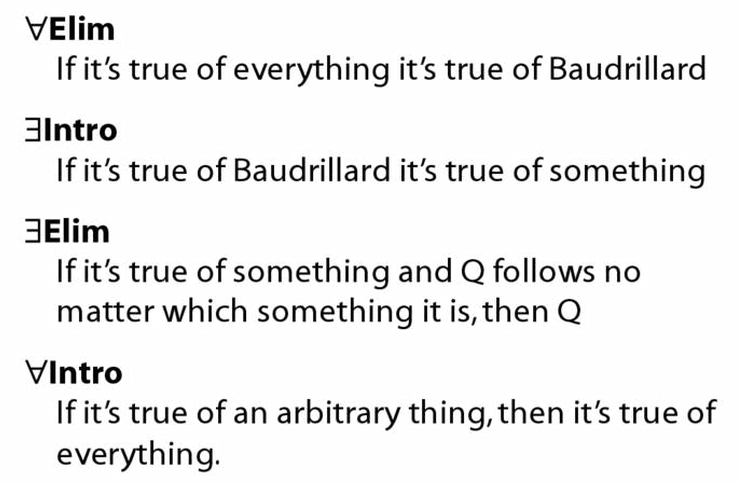
\includegraphics[scale=0.3]{img/quantifier_rule_summary.png}
\end{center}
 
\columnbreak 
\section{Scope and Quantifiers}
 
\emph{Reading:} §9.5, §9.6
 
\begin{minipage}{\columnwidth}
 
Underlining shows the scope of the quantifiers:
 
\begin{center}
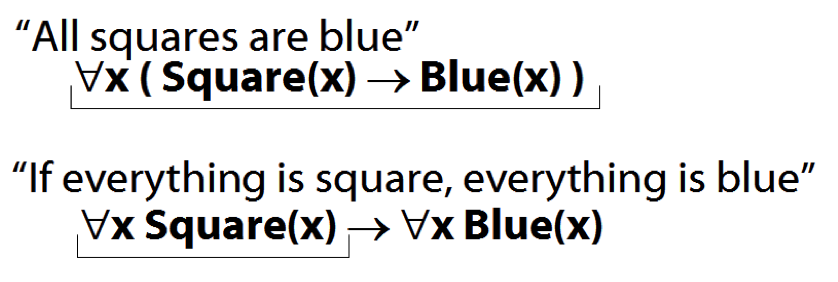
\includegraphics[scale=0.3]{img/scope_quantifiers.png}
\end{center}
\end{minipage}
 
 
 
\section{Translation with Quantifiers}
 
\emph{Reading:} §9.5, §9.6
 
\begin{minipage}{\columnwidth}
 
All discordians weep:
 
∀x( Dscrdn(x) → Wps(x) )
 
\end{minipage}
 
\begin{minipage}{\columnwidth}
 
All \textbf{French} discordians weep:
 
∀x( ( \textbf{Frnch(x) ∧} Dscrdn(x) ) → Wps(x) )
 
\end{minipage}
 
\begin{minipage}{\columnwidth}
 
All French discordians weep \textbf{and wail}:
 
∀x( ( Frnch(x) ∧ Dscrdn(x) ) → ( Wps(x) \textbf{ ∧ Wls(x)} ) )
 
\end{minipage}
 
\begin{minipage}{\columnwidth}
 
All French discordians weep and wail \textbf{except Gillian Deleude}:
 
∀x( ( Frnch(x) ∧ Dscrdn(x) \textbf{∧ ¬(x=a)} ) → ( Wps(x) ∧ Wls(x) ) )
 
\end{minipage}
 
 
 
\columnbreak  
\section{What does ∃ mean?}
 
We give the meaning of ∃ by specifying what it takes for a sentence containing ∃ to be true:
 
\begin{enumerate}
 
\item Give every object a name.
 
\item For each name in turn, create a new sentence like this: delete the quantifier and replace all instances of the variable it binds with that name.
 
\item If ANY of the new sentences are true, so is the original sentence.
 
\end{enumerate}
 
 
 
\section{Quantifiers Bind Variables}
 
\emph{Reading:} §9.3
 
\begin{center}
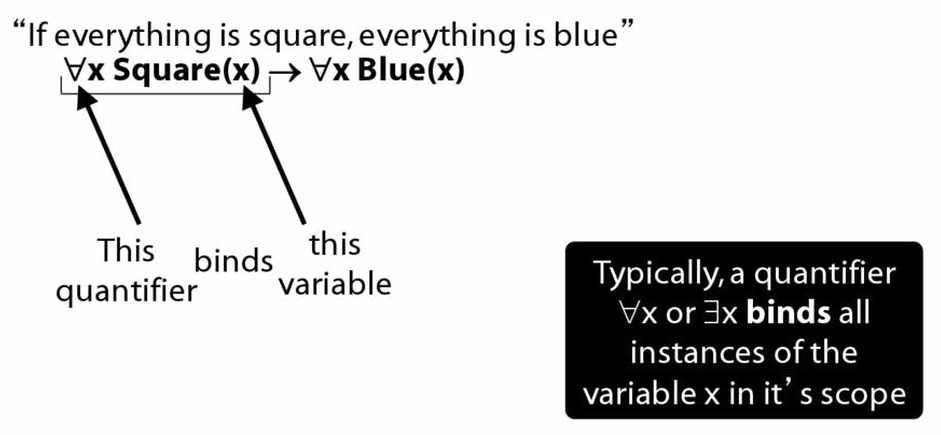
\includegraphics[scale=0.3]{img/quantifiers_scope.png}
\end{center}
 
\columnbreak 
\section{Substitution of Equivalents}
 
\emph{Reading:} §4.5, §10.3
 
Suppose that φ, ψ and χ are sentences of FOL. Suppose that φ is logically equivalent to ψ. Let χ[φ/ψ] be the result of replacing, in χ, zero or more occurrences of φ with ψ. The \emph{subsitution theorem} says that χ[φ/ψ] is logically equivalent to χ.
 
 
 
\section{Fubar Rules}
 
\emph{Reading:} §8.3
 
\begin{minipage}{\columnwidth}
 
Consider this made-up rule:
 
\begin{center}
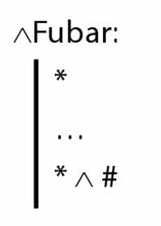
\includegraphics[scale=0.3]{img/fubar_rule.png}
\end{center}
Q1. What would be wrong with adding ∧Fubar to Fitch?
 
Q2. What would be wrong with having ∧Fubar in any system of proof?
 
\end{minipage}
 
 
 
\section{Something Is Above Something}
 
\emph{Reading:} §11.1
 
\begin{minipage}{\columnwidth}
 
Something is above something:
 
∃x ∃y Above(x,y)
 
\end{minipage}
 
 
 
\section{Two Things Are Broken}
 
\emph{Reading:} §14.1
 
To translate sentences involving number into FOL, use identity. For example,
 
`Two things are broken' might be translated as:
 
∃x ∃y ( Broken(x) ∧ Broken(y) ∧ ¬(x=y) )
 
 
 
\section{Does ‘if’ mean what ‘→’ means?}
 
\emph{Reading:} §7.3
 
 
These two arguments are valid: does that mean that `if' means what `→' means?
 
\begin{center}
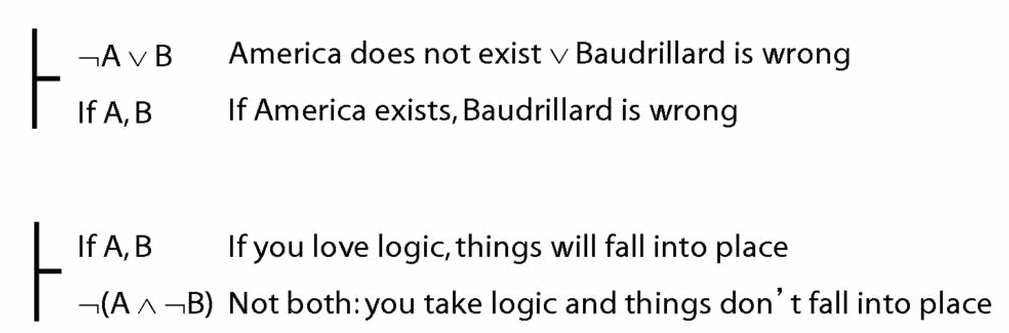
\includegraphics[scale=0.3]{img/if_is_arrow.png}
\end{center}
 
 
The English argument isn't valid; the FOL argument is valid; therefore `if' can't mean what `→' means?
 
\begin{center}
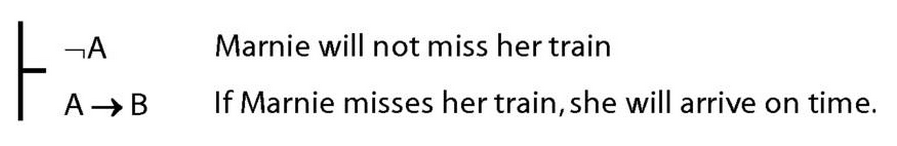
\includegraphics[scale=0.3]{img/if_aint_arrow.png}
\end{center}
 
\vfill
\begin{minipage}{\columnwidth}
\section{Exercises}
These exercises will be discussed in seminars the week after this lecture.
The numbers below refer to the numbered exercises in the course textbook, e.g.\ `1.1' refers to exercise 1.1. on page 39 of the second edition of \emph{Language, Proof and Logic}. Exercises marked `*' are optional.
 
\begin{quote}
8.26--8.30
 
9.8–-9.10
 
9.16.10--9.16.15
 
9.17.7--9.17.15
 
10.20
 
*10.24--10.7
 
10.28--10.29
 
13.2--13.3, 13.8--13.9
 
13.11, 13.13, 13.15
 
9.12-–9.13
 
4.31, 7.25
 
\end{quote}
\end{minipage}

%--- end paste
%--------------- 
 

\end{multicols*}

\end{document}